
% ════════════════════════════════════════════
% 模型准备（5.3.2.模型准备.tex，三级子块）
% ════════════════════════════════════════════
\subsubsection{模型准备}

\textbf{1.数据预处理}

附件三给出了 2025 年全年每天 0:00、6:00、12:00、18:00 四个时刻发布的未来 24 小时整点光伏发电功率预报，而实际负载与光伏功率的时间分辨率均为 10 分钟，因此需要将小时分辨率的光伏预报插值到 10 分钟间隔上。设某预报时刻 $\tau$ 发布的第 $n$ 小时预报功率为 $f_n$，其对应时刻为 $\tau+n$（小时），则预报序列在小时尺度上给出了一组离散点 $(\tau,f_0),(\tau+1,f_1),\dots,(\tau+24,f_{23})$。对第 $k$ 个间隔末端时刻 $t_k=(k+1)/6$（小时）进行线性插值，得到：
\begin{equation}
    S^{\tau}_k=\mathrm{interp}\big(t_k;\,\{\tau+j\}_{j=0}^{24},\,\{f_{j-1}\}_{j=1}^{24}\big)
\end{equation}
其中，$f_0$ 取 $f_1$ 近似当前整点功率，$S^{\tau}_k$ 为预报时刻 $\tau$ 发布的第 $k$ 个间隔的光伏预报功率。各预报时刻的实际预报与真实光伏对比如图\ref{fig:preprocess3}所示。

\begin{figure}[H]
    \centering
    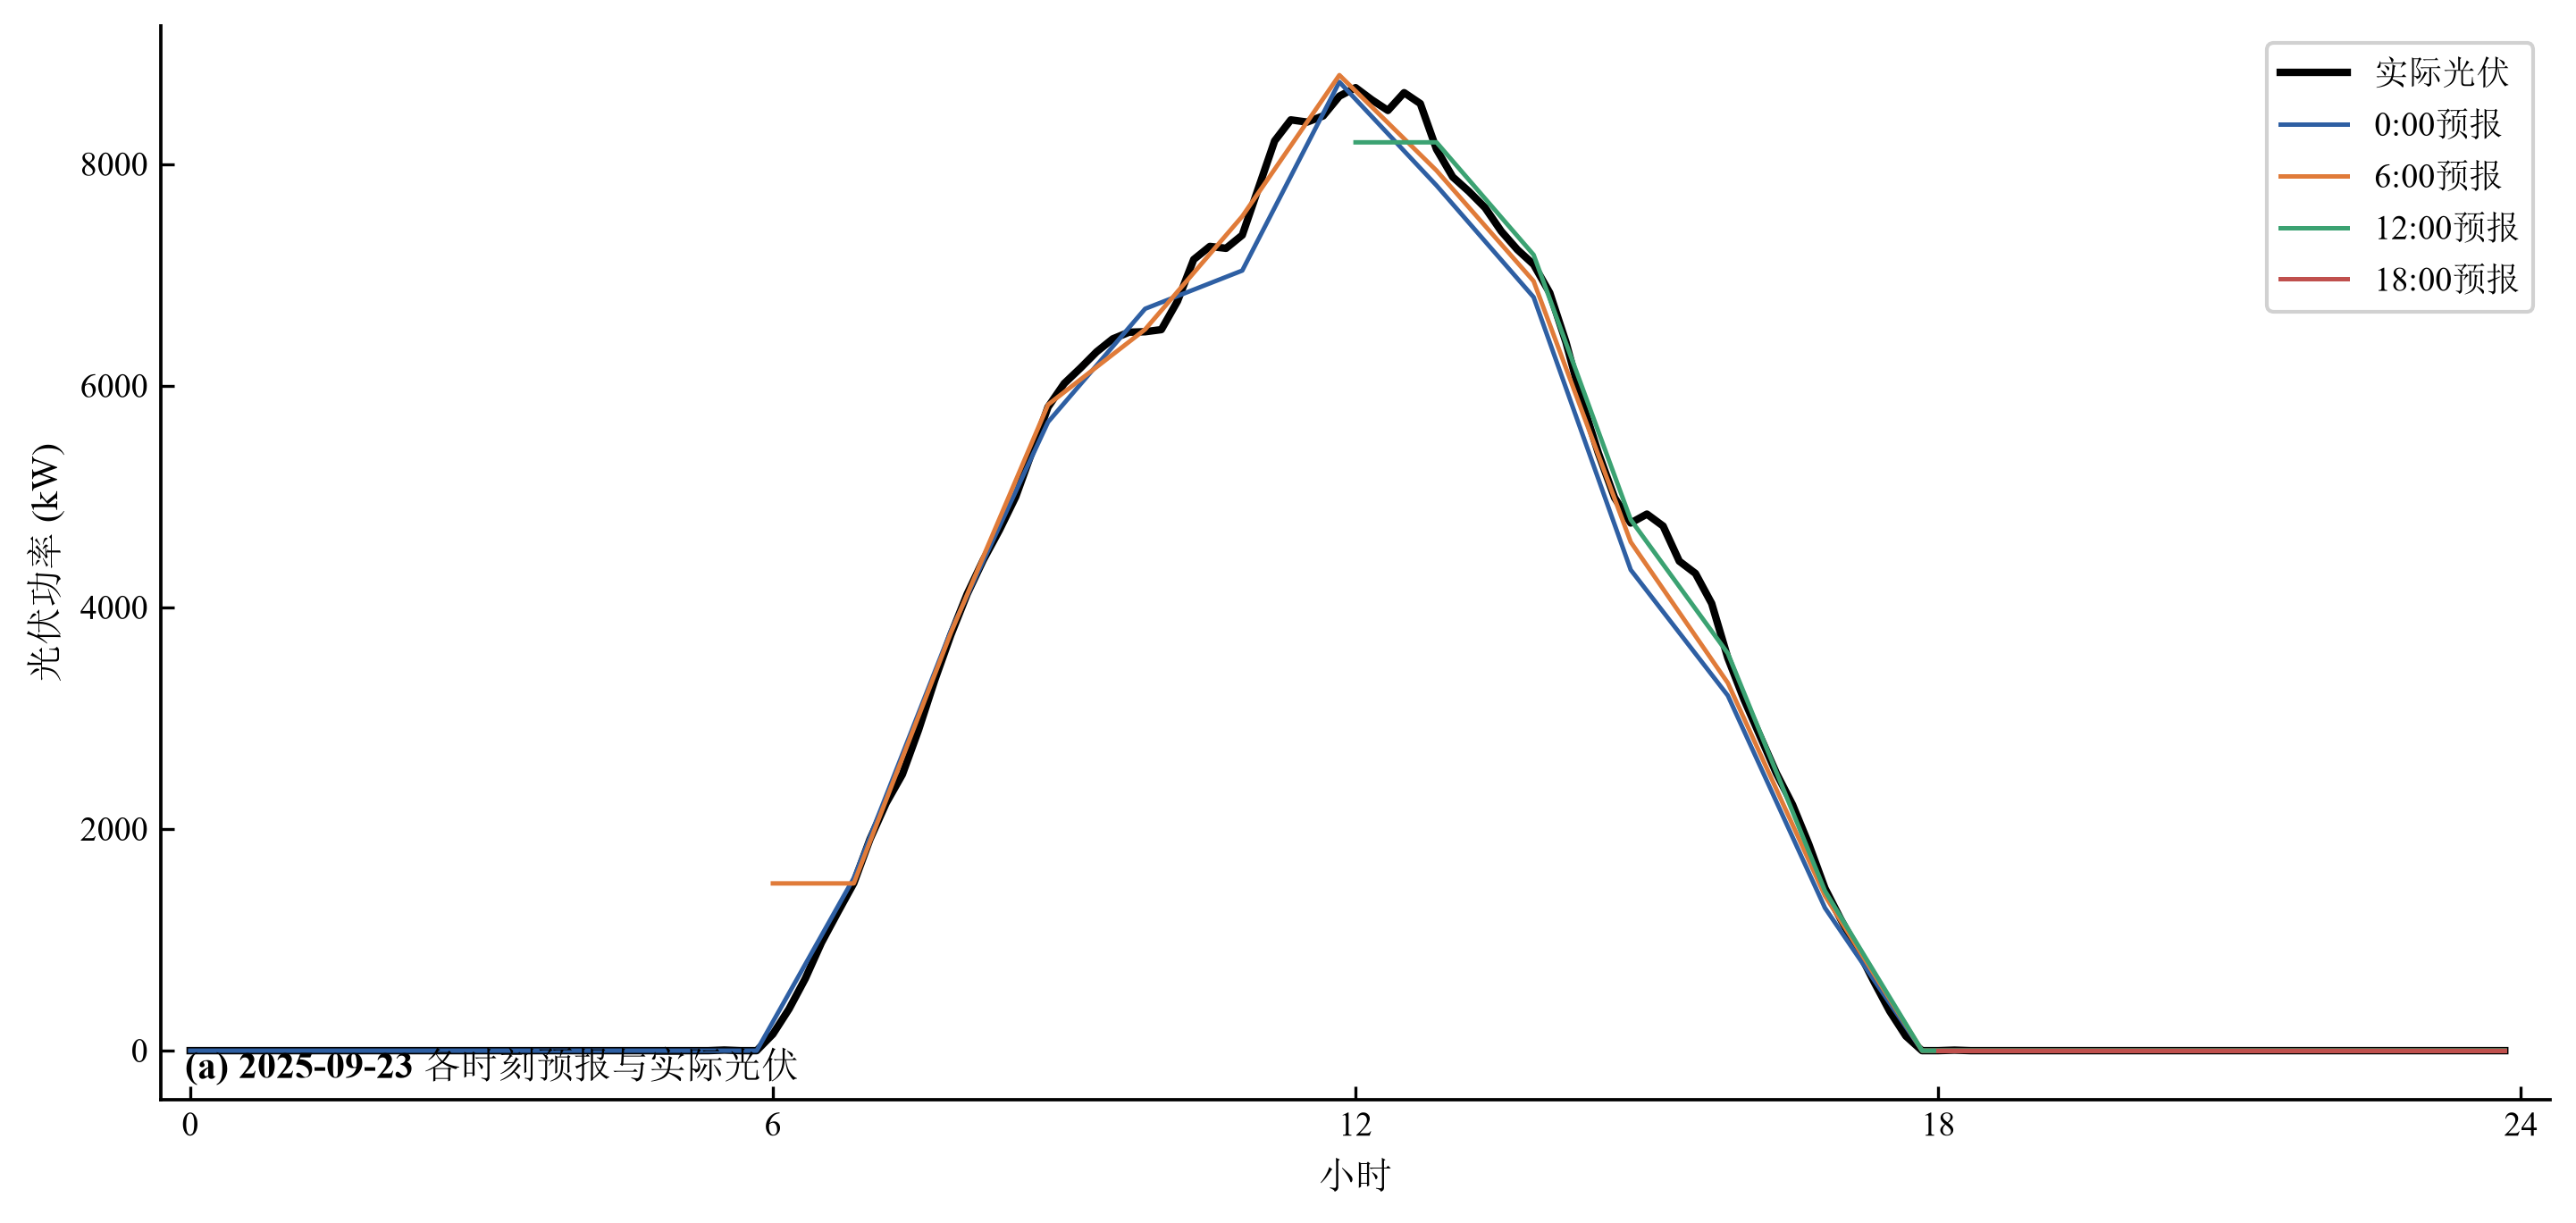
\includegraphics[width=0.70\textwidth]{求解/问题三/图片/图3-1_预报与实际光伏对比.png}
    \caption{各预报时刻的光伏预报与真实光伏对比}
    \label{fig:preprocess3}
\end{figure}

由图\ref{fig:preprocess3}可知，四个预报时刻的光伏预报均能刻画白天光伏功率的单峰形态，且越接近实际发生时刻发布的预报越贴近真实光伏，这与光伏功率预测误差随预测时域缩短而减小的规律一致\cite{antonanzas2016}，说明滚动利用最新预报能够有效降低预报误差，为调整购电策略提供了信息基础。

\textbf{2.算法选择}

在完成预报插值后，本问需要在滚动时域内求解带分段惩罚费用的优化问题。计划购电量与调整购电量的偏差费用是分段线性凸函数，可借助上境变量将其线性化后仍用线性规划求解。可从优化精度与计算效率两个维度比较动态规划与线性规划，如表\ref{tab:algo3}所示。

\begin{longtable}{>{\centering\arraybackslash}p{0.22\textwidth}>{\centering\arraybackslash}p{0.24\textwidth}>{\centering\arraybackslash}p{0.22\textwidth}>{\centering\arraybackslash}p{0.20\textwidth}}
  \caption{问题三算法对比}
  \label{tab:algo3} \\
  \toprule
  算法 & 分段费用处理 & 全局最优性 & 计算效率 \\
  \midrule
  \endfirsthead
  \caption{问题三算法对比（续）} \\
  \toprule
  算法 & 分段费用处理 & 全局最优性 & 计算效率 \\
  \midrule
  \endhead
  \bottomrule
  \endfoot
  动态规划 & 需离散化 & 近似 & 一般 \\
  线性规划 & 上境变量线性化 & 严格保证 & 高 \\
\end{longtable}

如\ref{tab:algo3}所示，动态规划需对连续购电量离散化，精度受步长限制；而分段凸费用可用上境变量精确线性化，再交给线性规划求解器求得全局最优解。综合以上分析，本问选择基于上境变量线性化的滚动线性规划策略进行求解。
